\documentclass[a4paper, 12pt]{article} %Formato de plantilla que vamos a utilizar
\usepackage[utf8]{inputenc}
\usepackage[spanish]{babel}
\usepackage[a4paper, total={6.5in, 9.5in}]{geometry}
\usepackage{graphicx} % Insertar imagenes
\usepackage[table,xcdraw]{xcolor} % Deteccion de colores
\usepackage{fancyhdr} % Crear cabeceros
\usepackage[colorlinks=true,linkcolor=blue]{hyperref} % Enlances
\usepackage{listings} % Bloques de código

% Declaracion de colores
\definecolor{colorTitulo}{HTML}{0F52BA}
\definecolor{codegreen}{rgb}{0,0.6,0}
\definecolor{codegray}{rgb}{0.5,0.5,0.5}
\definecolor{codepurple}{rgb}{0.58,0,0.82}
\definecolor{backcolour}{rgb}{0.95,0.95,0.92}

% Declaracion de variables
\newcommand{\logoPunta}{img/LogoPuntaDelVerde.png} % Logo del punta
\newcommand{\logoKeter}{img/logo.png} % Logo de la practica
\newcommand{\nombrePractica}{Keter Vulnerability} % Nombre de la practica
\newcommand{\bigpar}{\par\vspace*{0.6cm}}

% Bloques de código
\lstdefinestyle{mystyle}{
    backgroundcolor=\color{backcolour},   
    commentstyle=\color{codegreen},
    keywordstyle=\color{magenta},
    numberstyle=\tiny\color{codegray},
    stringstyle=\color{codepurple},
    basicstyle=\ttfamily\footnotesize,
    breakatwhitespace=false,         
    breaklines=true,                 
    captionpos=b,                    
    keepspaces=true,                 
    numbers=left,                    
    numbersep=5pt,                  
    showspaces=false,                
    showstringspaces=false,
    showtabs=false,                  
    tabsize=2
}

\lstset{style=mystyle}

% Header y footer
\pagestyle{fancy}
\fancyhf{}
\rhead{\includegraphics[width=15cm]{\logoPunta}}
\rfoot{Keter Vulnerability\par Página \thepage}
\lfoot{Emilio Sanchez Garcia\par 2º ASIR}
\renewcommand{\headrulewidth}{0pt}
\renewcommand{\footrulewidth}{1pt}
\setlength\headheight{40.62811pt} % quitar aviso cabecero
\addtolength{\topmargin}{-0.62811pt}

% Comienzo del documento
\begin{document}
% Portada
\begin{titlepage}
	\centering
	\includegraphics[width=0.3\textwidth]{\logoKeter}\bigpar
	{\LARGE \textbf{Proyecto Final}\par\vspace{0.2cm}}
	{\Huge\bfseries\textcolor{colorTitulo}{\nombrePractica}}
\end{titlepage}

% Indice
\tableofcontents

% Documentacion
\newpage
\textcolor{colorTitulo}{\section{Introducción Teórica}}

\textbf{Keter Vulnerability} es una página web diseñada para representar algunos
errores de configuración a la hora de crear aplicaciones web. El objetivo es disponer a
los usuarios de diferentes \textbf{retos} donde deberán usar sus conocimientos y su capacidad de
búsqueda a través de Internet para explotar dichas vulnerabilidades.\bigpar

\begin{figure}[hbt]
	\centerline{
\includegraphics[width=1\textwidth]{img/vuln.png}}
	\caption[Vulnerability imagen]{Fuente \href{https://whiteknightit.com/2019/09/18/xeon-and-other-intel-cpus-hit-by-netcat-security-vulnerability/}{whiteknightit.com}}
\end{figure}

El objetivo es ser capaces de concienciar a jóvenes \textbf{desarrolladores} del peligro que puede
llevar realizar páginas web sin conciencia sobre los errores. Al final veremos como el usuario
es un factor bastante peligroso para los desarrolladores y como nunca podemos confiar plenamente
en sus intenciones.\par
Es por ello que debemos protegernos con las últimas tecnologías. Mantenernos \textbf{actualizados y
	activos} será la clave para evitar cualquier error.\bigpar

El objetivo de esta página es su escalabilidad. Una vez terminado el proyecto la página pasará a ser código abierto,
con el objetivo de que la comunidad pueda aportar sus propios retos y módulos desde GitHub. Es por ello que gran parte
de los contenidos serán en inglés.
\newpage

Haremos uso de las últimas tecnologías para la realización de este proyecto:
\begin{itemize}
	\item \textbf{LaTex}: haremos uso de esta herramienta de texto mediante código para la creación de esta misma documentación.
	\item \textbf{NodeJS}: utilizaremos este paquete de recurso para la creación de la página web.
	\item \textbf{Mongo Atlas}: nos prooverá una base de datos principal para retos de NoSQL Injection.
	\item \textbf{HerokuApps}: será la página que hosteará nuestra aplicación.
	\item \textbf{GitHub}: allí subiremos el código y utilizaremos la función de GitHub Pages para crear una pequeña página web que muestre un breve resumen.
	\item \textbf{Docker}: crearemos un proyecto adicional con un contenedor en Docker para poder montar y utilizar nuestra aplicación en local.
\end{itemize}
\begin{figure}[hbt]
	\raggedright{
\includegraphics[width=0.16\textwidth]{img/latex.png}}
	\raggedright{
\includegraphics[width=0.16\textwidth]{img/node.png}}
	\raggedright{
\includegraphics[width=0.16\textwidth]{img/mongo.png}}
	\raggedright{
\includegraphics[width=0.16\textwidth]{img/heroku.png}}
	\raggedright{
\includegraphics[width=0.16\textwidth]{img/github.png}}
	\raggedright{
\includegraphics[width=0.16\textwidth]{img/docker.png}}
\end{figure}
\clearpage


\textcolor{colorTitulo}{\section{Introducción Técnica}}


\clearpage


\textcolor{colorTitulo}{\section{API}}


\clearpage


\textcolor{colorTitulo}{\section{APP}}

La app \textbf{Keter Vulnerability} está creada mediante Typescript, compilada en JavaScript. Utiliza el
framework de \textbf{Angular}, junto a \textbf{Angular Material} y \textbf{Bootstrap}.
\bigpar

\subsection{Rutas}
Para poder tener una mayor optimización he separado las distintas rutas, de esta forma tan solo cargarán
unas páginas dependiendo de en que parte de la aplicación se encuentre.
\begin{figure}[hbt]
	\centerline{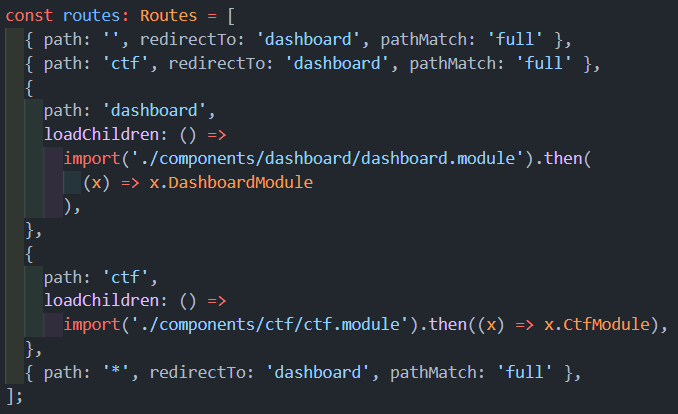
\includegraphics[width=1\textwidth]{img/app/15-17-32-36.png}}
	\caption[Rutas]{rutas principales.}
\end{figure}
Estas rutas son las primeras, se encuentran en el archivo por defecto creado por Angular.\par
La primera declaración redirige al \textbf{dashboard} cualquier ruta vacia. La segunda redirige la ruta
\textbf{ctf} al dashboard igualmente.
La siguiente ruta es la del dashboard, en vez de cargar entero el dashboard y todos sus componentes cargamos
únicamente la propia página, de igual manera que hacemos con el \textbf{ctf}.\newpage
Veremos a continuación las rutas del dashboard:\par
\begin{figure}[hbt]
	\centerline{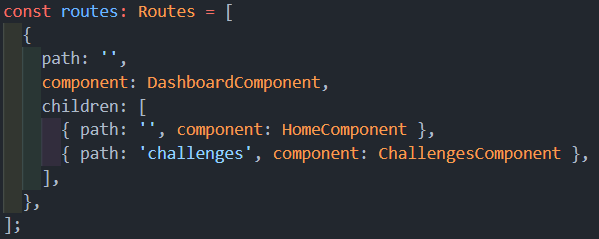
\includegraphics[width=1\textwidth]{img/app/15-17-49-27.png}}
	\caption[Rutas]{rutas hijas del Dashboard.}
\end{figure}
Estas rutas son cargadas únicamente cuando se ingresa al Dashboard. De esta forma podemos tener la app
dividida en dos partes. Por otro lado el \textbf{ctf} tiene su propio archivo de rutas del que parten los demás
componentes, esto nos permite ahorrar la carga de todos los retos cuando tan solo hemos entrado al Dashboard.
De igual manera, mientras nos encontremos en un reto no tendremos el Dashboard cargando también.\newpage

\subsection{Módulos}
Hemos separado también los módulos para una carga más rápida. Mantenemos el archivo por defecto de los módulos
pero importamos un nuevo módulo que hemos creado nosotros: \textbf{Shared}.\par
\begin{figure}[hbt]
	\centerline{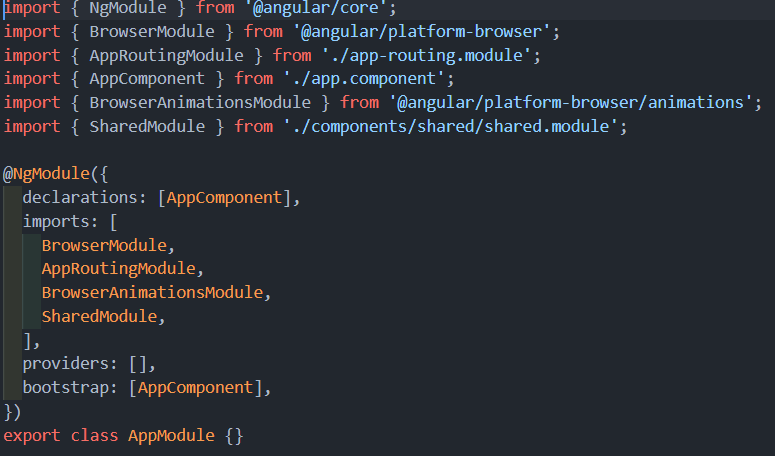
\includegraphics[width=1\textwidth]{img/app/15-17-53-17.png}}
	\caption[Modulos]{\textbf{app.module.ts} por defecto.}
\end{figure}
En dicho módulo \textbf{Shared} importamos todos los módulos que usamos para el proyecto, de esta forma podemos dividir
los archivos y tener un mayor control de errores.\newpage

\subsection{DOMsanitizer}
Angular por defecto viene protegido contra ciertas vulnerabilidades, para poder recrearlas ha sido necesario escapar
algunos de estas protecciones, como por ejemplo \textbf{DOMsanitizer}.
\begin{figure}[hbt]
	\centerline{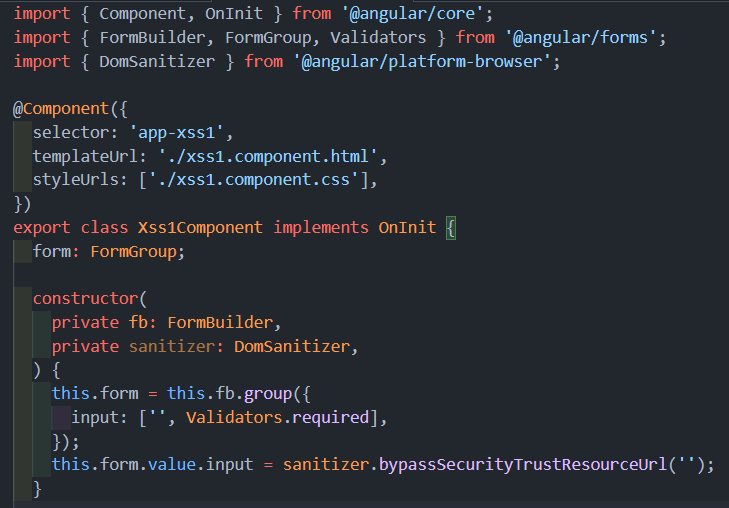
\includegraphics[width=1\textwidth]{img/app/15-18-06-57.png}}
	\caption[Modulos]{desactivar DOMsanitizer.}
\end{figure}
Para poder escapar la seguridad lo primero que haremos será usar los formularios de Angular para poder
tomar el valor en una variable. Importaremos la librería de DOMsanitizer y estableceremos el valor
como fiable, de esta forma podremos explotar algunas vulnerabilidades, como XSS.
\clearpage


\textcolor{colorTitulo}{\section{Vulnerabilidades utilizadas}}

\subsection{XSS}
Cross-Site Scripting son un tipo de ataque mediante inyección, mediante el cual código malicioso es inyectado
en páginas confiables. Los ataques de XSS ocurren cuando el atacante usa una aplicación web para enviar
código malicioso, generalmente en forma de script de navegador, para un tercer usuario. Puede ocurrir en multitud
de aplicaciones web mediante la entrada de un usuario, sin validar o codificar su valor.\bigpar
\begin{footnotesize}
	Fuente: \href{https://owasp.org/www-community/attacks/xss/}{OWASP Cross Site Scripting (XSS)}
\end{footnotesize}
\bigpar

\textbf{AÑADIR TIPOS}
\clearpage


\textcolor{colorTitulo}{\section{Explotaciones}}

\subsection{Send a comment!}
La explotación de este reto consiste en utilizar la vulnerabilidad de XSS Reflected.\par
Con tan solo poner un comando entre las etiquetas \textbf{<script>...</script>} nos dará por solucionado
el reto.\bigpar
\clearpage


\textcolor{colorTitulo}{\section{Posibles soluciones}}

\subsection{Send a comment!}
Para esta vulnerabilidad la solución consiste en depurar la entrada del usuario. En vez de usar
DOMsanitizer para desactivarlo, si no lo nombramos por defecto estaría activado. Por asegurarnos podemos
especificar que depure esa parte. Para ello debemos usar la siguiente estructura:
\begin{lstlisting}
this.form.value.input = sanitizer.sanitize('');
\end{lstlisting}
en sustitución del código que teniamos anteriormente:
\begin{lstlisting}
this.form.value.input = sanitizer.bypassSecurityTrustResourceUrl('');
\end{lstlisting}
\begin{footnotesize}
	\textbf{Nota:} DOMsanitizer tiene distintos formatos y funciones, no se limita únicamente a estas dos, por lo que
	en algunos casos puede ser mejor utilizar otras.
\end{footnotesize}

\clearpage


\textcolor{colorTitulo}{\section{Conclusión}}

\clearpage


\textcolor{colorTitulo}{\section{Fuentes}}

\large{Info}
\begin{itemize}
	\item \href{https://owasp.org}{OWASP}
	\item \href{https://angular.io/api/platform-browser/DomSanitizer}{Angular DOMsanitizer}
	\item 	\item \href{https://netbasal.com/angular-2-security-the-domsanitizer-service-2202c83bd90}{Angular DOMsanitizer by Netanel Basal}
\end{itemize}
\bigpar

\large{Github}
\begin{itemize}
	\item \href{https://github.com/angular}{Angular}
	\item \href{https://github.com/swisskyrepo/PayloadsAllTheThings}{PayloadsAllTheThings}
\end{itemize}
\bigpar

\large{Recursos}
\begin{itemize}
	\item \href{https://v7.material.angular.io/}{Angular Material}
\end{itemize}

\clearpage


\end{document}